% INFORMATION
Information-wise the estimation of the unknowns in \cref{eq:Multilevel:Model} can be based on the observed data \(\bm{y}_i\), the Bayesian prior \(\pi(\bm{\theta}_{\bm{X}})\),
the structural knowledge \(f_{\bm{X} \cond \bm{\Theta}_{\bm{X}}}(\bm{x}_i \cond \bm{\theta}_{\bm{X}})\) and the information encapsulated in \(f_{\bm{E}_i}(\bm{y}_i-\mathcal{M}(\bm{x}_i,\bm{d}_i))\).
% INDIVIDUAL INFERENCE
Now we focus on the optimal inference of an individual parameter \(\bm{x}_{\analyzed}\) for some \(\analyzed \in \{1,\ldots,n\}\).
Instead of merely inverting the observation \(\bm{y}_{\analyzed}\) for the corresponding \(\bm{x}_{\analyzed}\), we solve the joint multilevel problem.
As it turns out, in doing so one can obtain more information about \(\bm{x}_{\analyzed}\) than what is contained in \(\bm{y}_{\analyzed}\).
One can indirectly learn from the data \(\tuple{\bm{y}_{\notanalyzed}} = (\bm{y}_1,\ldots,\bm{y}_{\analyzed-1},\bm{y}_{\analyzed+1},\ldots,\bm{y}_n)\) that were collected in different experiments.
This is beneficial in the event of that the tests in experiment \(\analyzed\) are less informative, e.g.\ the associated data \(\bm{y}_{\analyzed}\) are less numerous or subject to a higher degree of measurement uncertainty.
In order to demonstrate the effect and to understand its underlying information flow, we pursue the following three strategies for the inference of \(\bm{x}_{\analyzed}\).

\subsection{Simple updating} \label{sec:Combination:Updating}
In this first approach inference of \(\bm{x}_{\analyzed}\) is based on the data \(\bm{y}_{\analyzed}\), the structural knowledge
\(f_{\bm{X} \cond \bm{\Theta}_{\bm{X}}}(\bm{x}_{\analyzed} \cond \bm{\theta}_{\bm{X}})\) and the prior \(\pi(\bm{\theta}_{\bm{X}})\).
By marginalizing the joint prior \(\pi(\bm{x}_{\analyzed},\bm{\theta}_{\bm{X}}) = f_{\bm{X} \cond \bm{\Theta}_{\bm{X}}}(\bm{x}_{\analyzed} \cond \bm{\theta}_{\bm{X}}) \, \pi(\bm{\theta}_{\bm{X}})\)
over the hyperparameters \(\bm{\theta}_{\bm{X}}\), the prior distribution of \(\bm{x}_{\analyzed}\) is written as
\begin{equation} \label{eq:MixturePrior}
  \pi(\bm{x}_{\analyzed}) = \int f_{\bm{X} \cond \bm{\Theta}_{\bm{X}}}(\bm{x}_{\analyzed} \cond \bm{\theta}_{\bm{X}}) \, \pi(\bm{\theta}_{\bm{X}}) \, \mathrm{d} \bm{\theta}_{\bm{X}}.
\end{equation}
This compound probability distribution represents the uncertainty of \(\bm{x}_{\analyzed}\) prior to data analysis.
Simple updating of the prior \(\pi(\bm{x}_{i_0})\) by conditioning on \(\bm{y}_{i_0}\) leads to the posterior \(\pi(\bm{x}_{i_0} \cond \bm{y}_{i_0})\).
While the observation \(\bm{y}_{\analyzed}\) has entered the analysis of \(\bm{x}_{\analyzed}\), the data \(\tuple{\bm{y}_{\notanalyzed}}\) have been neglected.
% DISCUSSION
In other words, the hierarchical problem structure has been recognized but it has not yet been fully utilized.
In constructing the prior \cref{eq:MixturePrior} it has been acknowledged that information about \(\bm{\theta}_{\bm{X}}\) carries information about \(\bm{x}_{\analyzed}\).
However, the uncertainty in \(\bm{\theta}_{\bm{X}}\) has not been reduced with further data \(\tuple{\bm{y}_{\notanalyzed}}\).
% DIMENSIONALITY
This simple updating approach establishes a \(m\)-dimensional inverse problem that is considered isolated from the remainder of the considered system,
% OTHER REALIZATIONS
i.e.\ if other realizations \(\bm{x}_i\) with \(i \neq \analyzed\) are of inferential interest, analogous yet separate inverse problems have to be solved.
% FIGURE: SIMPLE UPDATING
A DAG-based visualization of the described situation is provided in \cref{fig:SimpleUpdating}.
The flow of information towards \(\bm{x}_{\analyzed}\) moves along the conditional relationships.
\begin{figure}[ht]
  \centering
  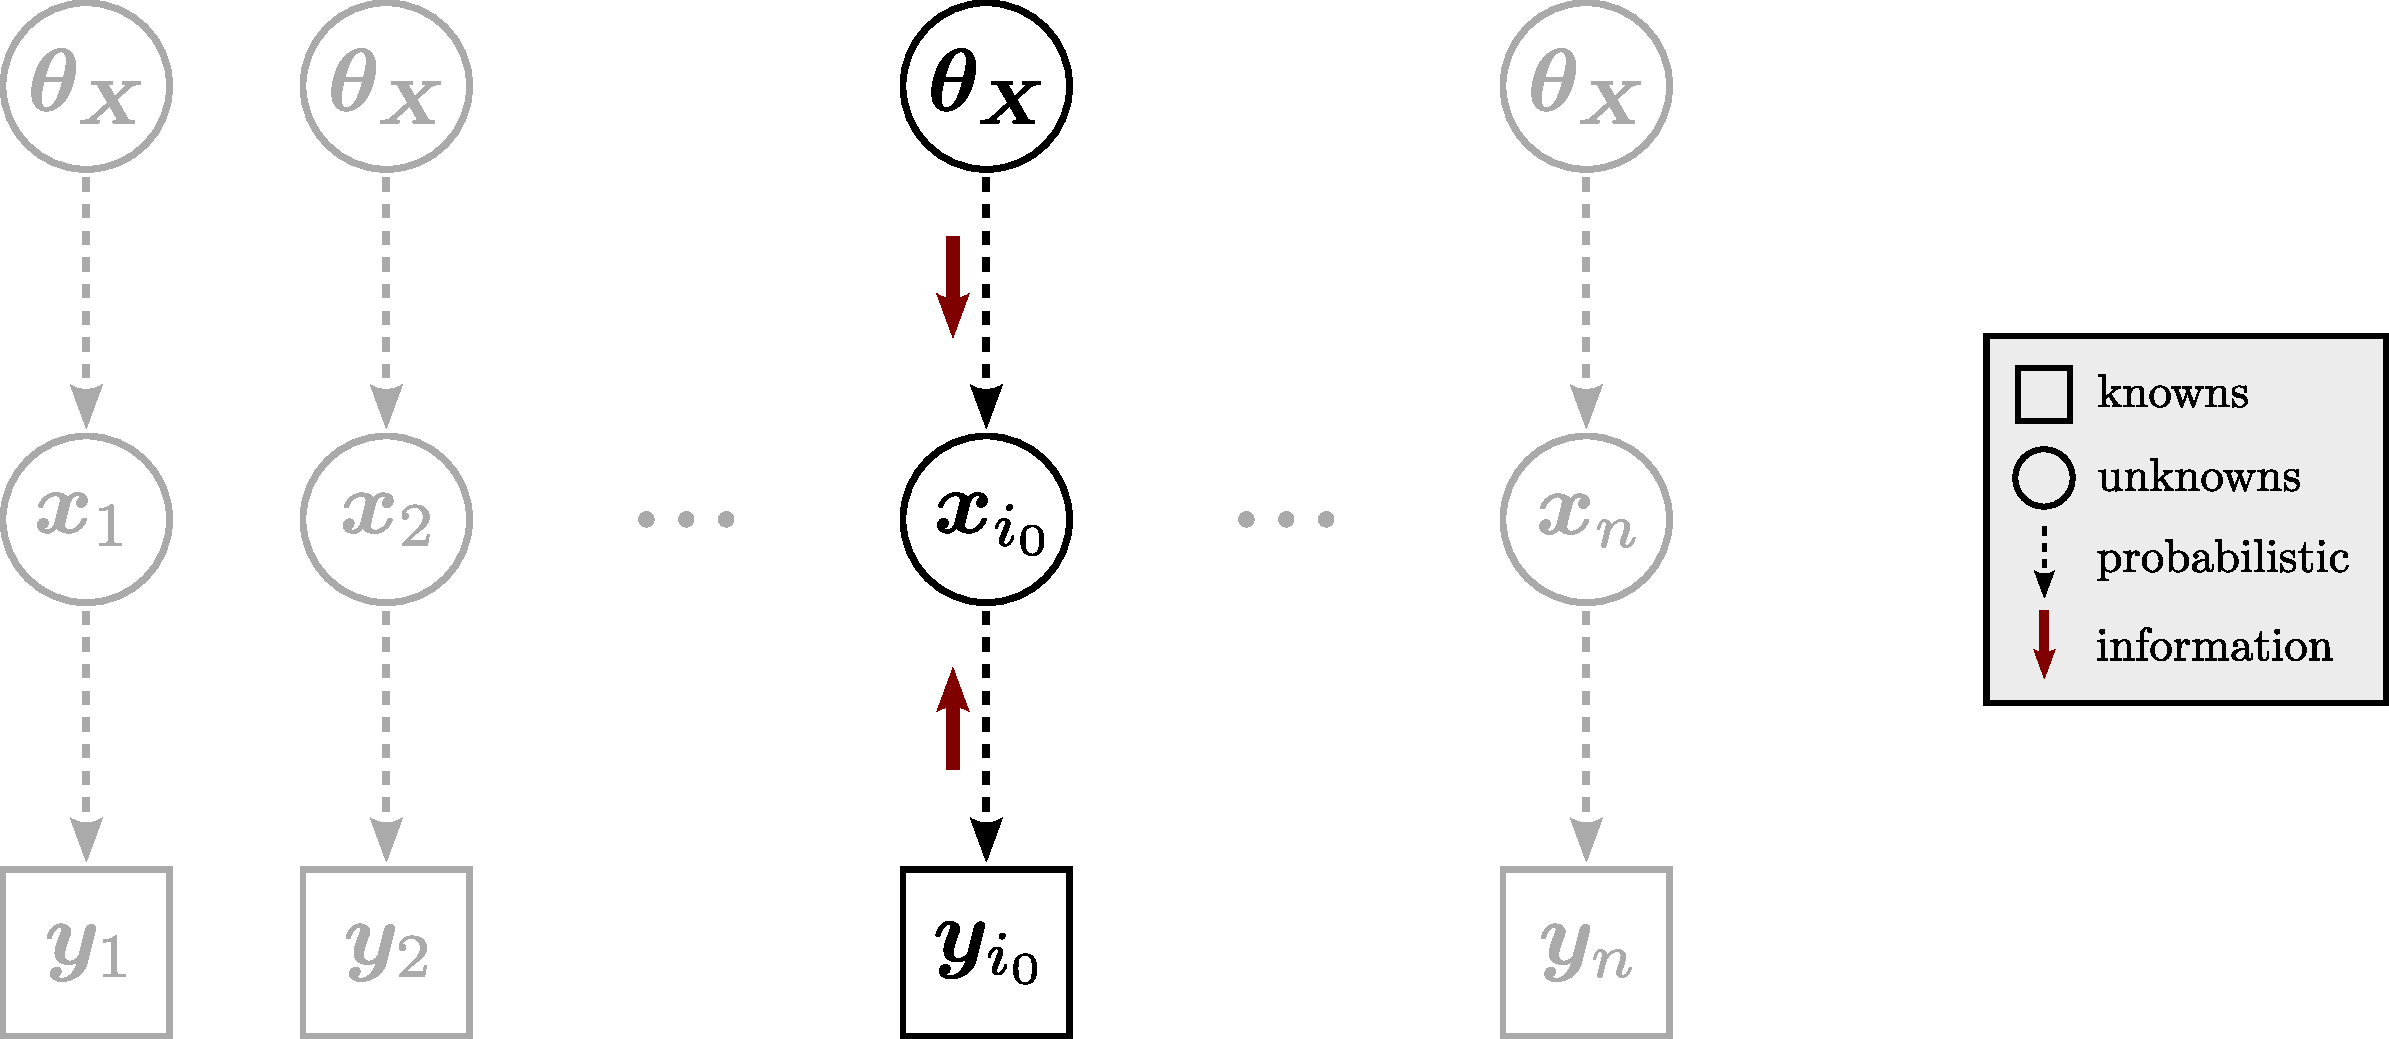
\includegraphics[height=\JRUESdagHeight]{fig_JRUES_Updating}
  \caption[Simple updating]{Simple updating.}
  \label{fig:SimpleUpdating}
\end{figure}

\subsection{Staged estimation} \label{sec:Combination:Filtering}
In the second approach the additional data that were disregarded above can be processed.
Initially the hyperparameters \(\bm{\theta}_{\bm{X}}\) are inferred by probabilistic inversion of the data \(\tuple{\bm{y}_{\notanalyzed}}\).
The posterior \(\pi(\bm{\theta}_{\bm{X}} \cond \tuple{\bm{y}_{\notanalyzed}})\) obtained in this first step can be translated into the distribution
\begin{equation} \label{eq:Filtering:Prior}
  \pi(\bm{x}_{\analyzed} \cond \tuple{\bm{y}_{\notanalyzed}})
  = \int f_{\bm{X} \cond \bm{\Theta}_{\bm{X}}}(\bm{x}_{\analyzed} \cond \bm{\theta}_{\bm{X}}) \, \pi(\bm{\theta}_{\bm{X}} \cond \tuple{\bm{y}_{\notanalyzed}}) \, \mathrm{d} \bm{\theta}_{\bm{X}}.
\end{equation}
It represents the uncertainty of \(\bm{x}_{\analyzed}\) following the analysis of \(\tuple{\bm{y}_{\notanalyzed}}\) but prior to analyzing \(\bm{y}_{\analyzed}\).
In a subsequent parameter estimation step \(\pi(\bm{x}_{\analyzed} \cond \tuple{\bm{y}_{\notanalyzed}}) \) can be interpreted as a prior.
The result of conditioning on \(\bm{y}_{\analyzed}\) is a posterior distribution \(\pi(\bm{x}_{\analyzed} \cond \tuple{\bm{y}_{\notanalyzed}},\bm{y}_{\analyzed})\).
% DISCUSSION
In a sequential way the estimation of \(\bm{x}_{\analyzed}\) has been based on the total number of data \(\tuple{\bm{y}_i}\).
% DIMENSIONALITY
In the first stage the posterior of \(\bm{\theta}_{\bm{X}}\) can be equivalently  computed as the solution to a \(l\)-dimensional inference problem with a marginalized likelihood
or as the marginal of the \((l + m \cdot (n-1))\)-dimensional multilevel posterior \(\pi(\tuple{\bm{x}_{\notanalyzed}},\bm{\theta}_{\bm{X}} \cond \tuple{\bm{y}_{\notanalyzed}})\).
The second stage involves \(m\)-dimensional Bayesian updating of \(\bm{x}_{\analyzed}\).
% PRIORS
The prior in \cref{eq:Filtering:Prior} that is used in the second step contains a lower degree of uncertainty with respect to \(\bm{x}_{\analyzed}\) than the one in \cref{eq:MixturePrior}.
In this sense it is a ``better'' prior.
% FIGURE: SEQUENTIAL FILTERING
The staged approach is visualized in \cref{fig:SequentialFiltering} where initial probabilistic inversion is shown on the left, i.e.\ information accumulates at \(\bm{\theta}_{\bm{X}}\).
The subsequent updating step is shown on the right, i.e.\ information about \(\bm{x}_{\analyzed}\) is extracted.
\begin{figure}[ht]
  \centering
  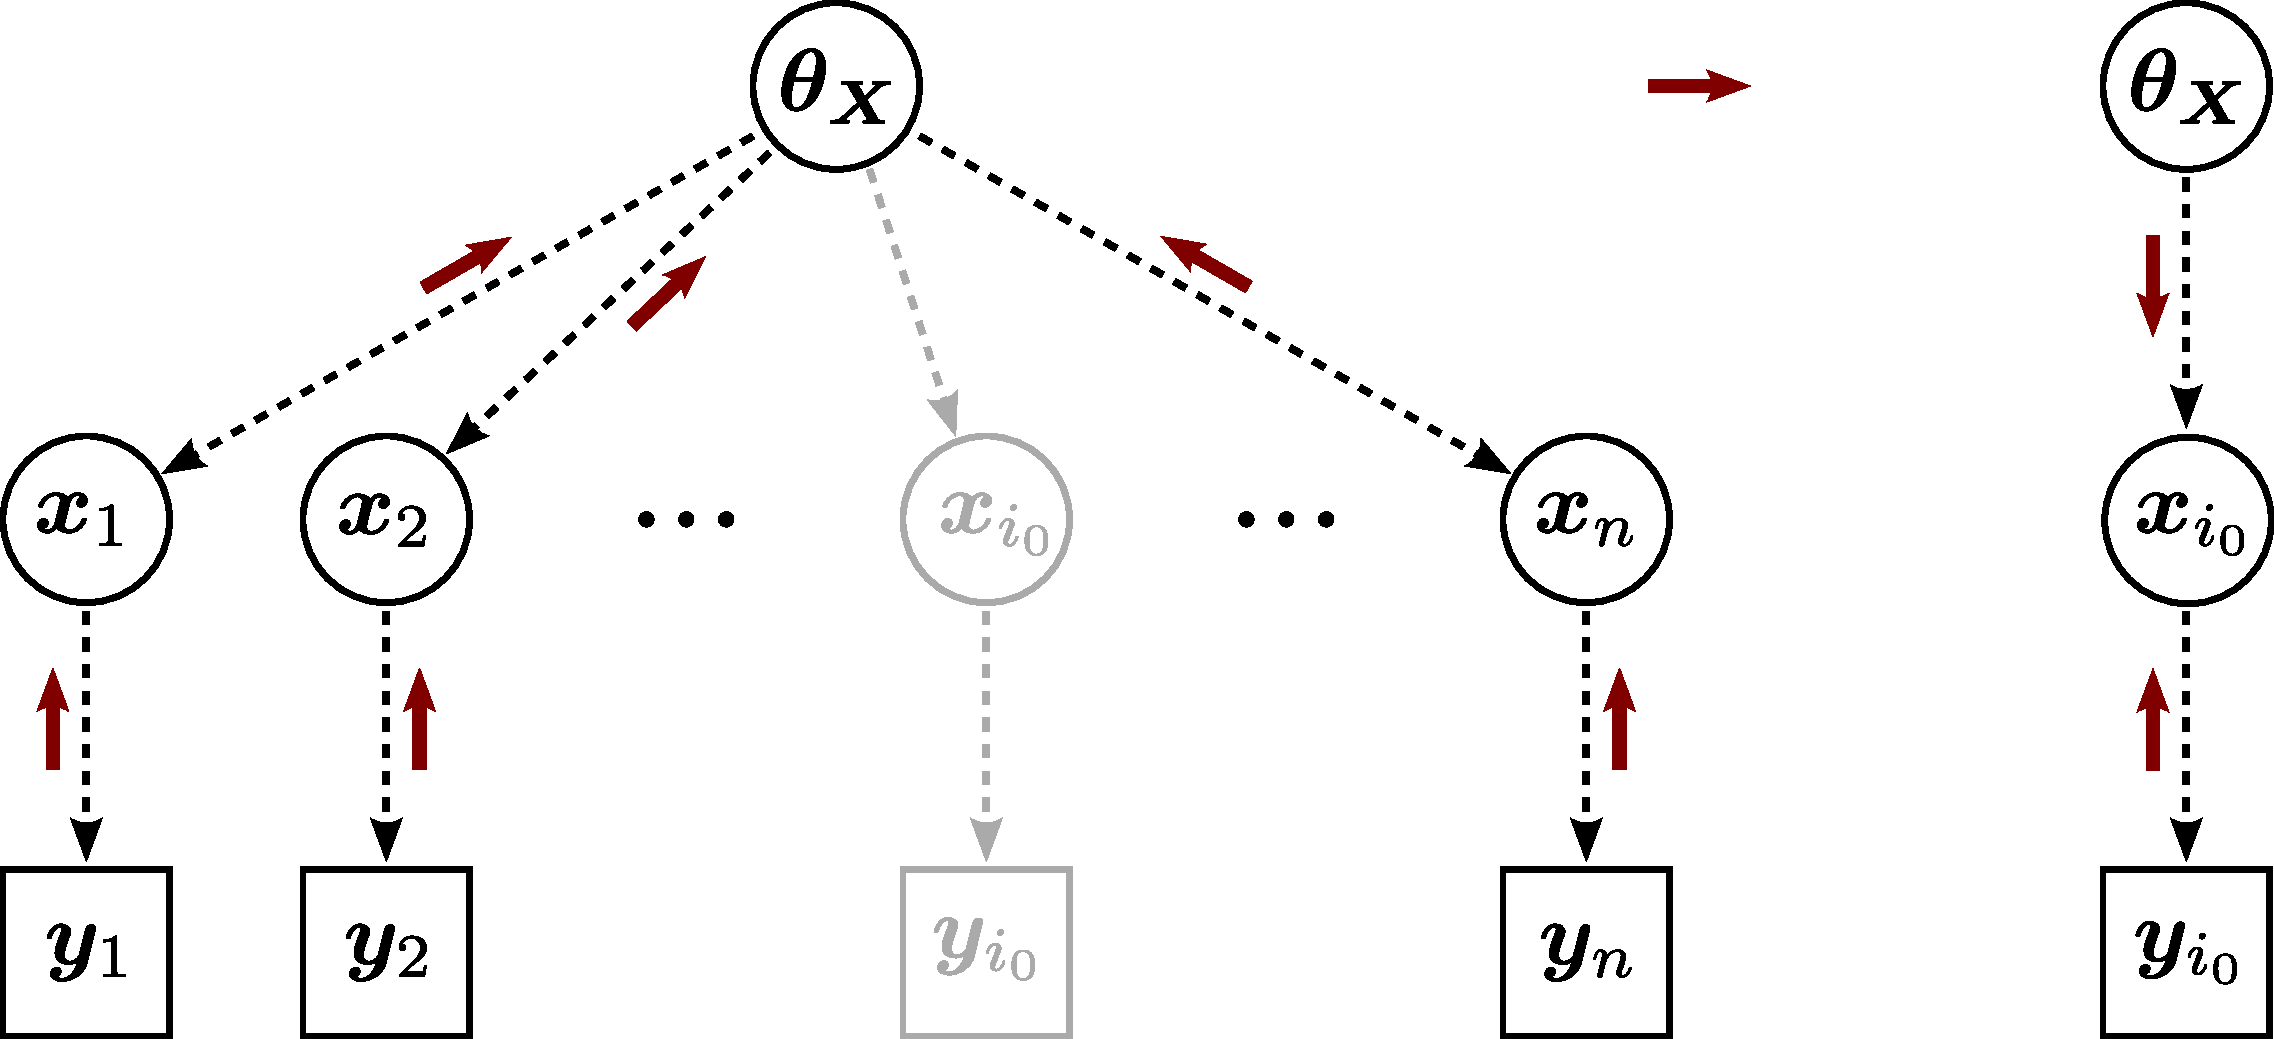
\includegraphics[height=\JRUESdagHeight]{fig_JRUES_Filtering}
  \caption[Staged estimation]{Staged estimation.}
  \label{fig:SequentialFiltering}
\end{figure}

\subsection{Multilevel inversion} \label{sec:Combination:Multilevel}
Multilevel analysis of \(\bm{x}_{\analyzed}\) is accomplished by constructing the joint posterior \(\pi(\tuple{\bm{x}_i},\bm{\theta}_{\bm{X}} \cond \tuple{\bm{y}_i})\) in \cref{eq:Multilevel:Posterior} and subsequently integrating out nuisance.
Since inferential attention is not focused on the parameters \(\tuple{\bm{x}_{\notanalyzed}}\) and hyperparameters \(\bm{\theta}_{\bm{X}}\), those are marginalized out.
The corresponding marginal of \(\bm{x}_{\analyzed}\) is
\begin{equation} \label{eq:Multilevel:MarginalPosterior}
  \pi(\bm{x}_{\analyzed} \cond \tuple{\bm{y}_i})
  = \idotsint \pi(\tuple{\bm{x}_i},\bm{\theta}_{\bm{X}} \cond \tuple{\bm{y}_i}) \, \mathrm{d}\bm{\theta}_{\bm{X}} \, \mathrm{d} \tuple{\bm{x}_{\notanalyzed}},
\end{equation}
where the simplifying notation \(\mathrm{d}\tuple{\bm{x}_{\notanalyzed}} = \mathrm{d}\bm{x}_1 \ldots \mathrm{d}\bm{x}_{\analyzed-1} \mathrm{d}\bm{x}_{\analyzed+1} \ldots \mathrm{d}\bm{x}_n\) is used.
% DISCUSSION
For estimating \(\bm{x}_{\analyzed}\) the available information has been processed as a whole.
Most notably the data \(\tuple{\bm{y}_{\notanalyzed}}\) have been utilized for reducing the posterior uncertainty of \(\bm{x}_{\analyzed}\).
% DIMENSIONALITY
In practice, if the \((l + m \cdot n)\)-dimensional posterior \(\pi(\tuple{\bm{x}_i},\bm{\theta}_{\bm{X}} \cond \tuple{\bm{y}_i})\) is computed via an appropriate sampler,
the marginal \(\pi(\bm{x}_{\analyzed} \cond \tuple{\bm{y}_i})\) can be easily extracted by considering the corresponding \(\bm{x}_{\analyzed}\)-components only.
The integral in \cref{eq:Multilevel:MarginalPosterior} does not have to be computed explicitly.
% OTHER REALIZATIONS
This way also other posterior marginals are obtained as a side product.
Notwithstanding that the hyperparameters \(\bm{\theta}_{\bm{X}}\) and realizations \(\bm{x}_i\) other than \(\bm{x}_{\analyzed}\) are not of immediate interest, they are incidentally inferred.
% FIGURE: MULTILEVEL INVERSION
In \cref{fig:MultilevelInversion} a DAG-based illustration of the flow of information that governs the inference of \(\bm{x}_{\analyzed}\) is shown.
% DISCUSSION
We remark that staged estimation and multilevel inversion formally resemble the Bayesian variants of filtering and smoothing \cite{Bayesian:Sarkka2013}, respectively, i.e.\ concepts from data assimilation in dynamical systems.
\begin{figure}[ht]
  \centering
  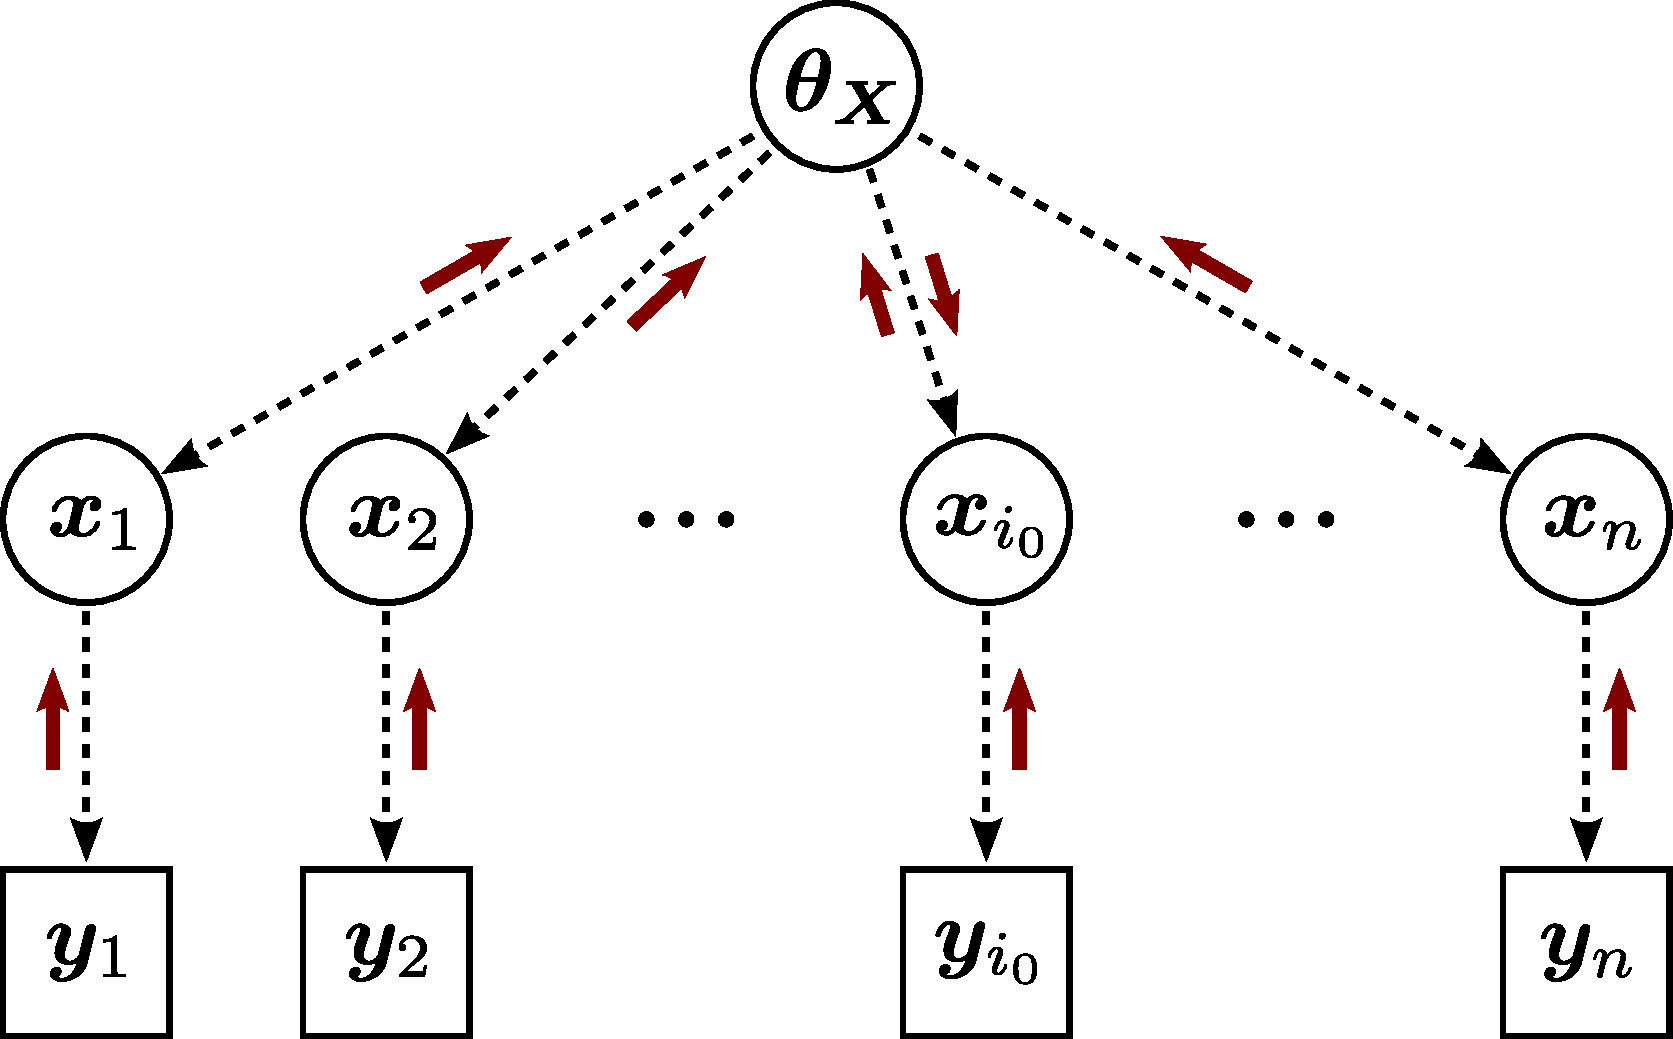
\includegraphics[height=\JRUESdagHeight]{fig_JRUES_Multilevel}
  \caption[Multilevel inversion]{Multilevel inversion.}
  \label{fig:MultilevelInversion}
\end{figure}